% Author: Rasmus Pank Roulund
\documentclass{minimal}
\usepackage{tikz}
\usepackage{verbatim}
\usetikzlibrary{calc,trees,positioning,arrows,chains,shapes.geometric,%
    decorations.pathreplacing,decorations.pathmorphing,shapes,%
    matrix,shapes.symbols}
\tikzset{
>=stealth',
  punktchain/.style={
    rectangle, 
    rounded corners, 
    % fill=black!10,
    draw=black, very thick,
    text width=8em, 
    minimum height=3em, 
    text centered, 
    on chain},
  line/.style={draw, thick, <-},
  element/.style={
    tape,
    top color=white,
    bottom color=blue!50!black!60!,
    minimum width=8em,
    draw=blue!40!black!90, very thick,
    text width=10em, 
    minimum height=3.5em, 
    text centered, 
    on chain},
  every join/.style={->, thick,shorten >=1pt},
  decoration={brace},
  tuborg/.style={decorate},
  tubnode/.style={midway, right=2pt},
}
\begin{document}
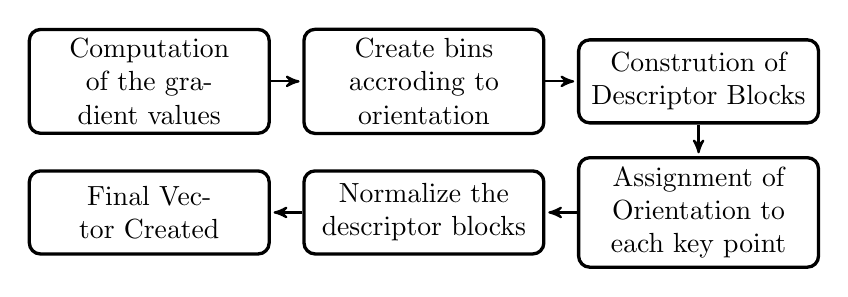
\begin{tikzpicture}
  [node distance=.4cm,
  start chain=going below,]
\node[punktchain, join=by {->}]{Computation of the gradient values};
\node[punktchain, on chain=going right, join=by {->}] (investeringer) {Create bins accroding to orientation};
\node[punktchain, on chain=going right, join,] (disk) {Constrution of Descriptor Blocks} ;
\node[punktchain, on chain=going below,join,] (risiko) {Assignment of Orientation to each key point};
\node[punktchain, on chain=going left, join=by {->},]  (makro) {Normalize the descriptor blocks};
\node[punktchain, on chain=going left, join=by {->}] (konk) {Final Vector Created};
  \end{tikzpicture}
\end{document}